\section{A Short Introduction to Factor Graphs}
\label{sec:IntroductionToFactorGraphs}

We introduce factor graphs, a powerful tool for statistical modeling.  
Factor graphs can be used to describe a number of commonly used 
statistical models, such as hidden Markov models, Markov random 
fields, Kalman filters, and Bayes nets. 

Suppose that we are given a set of n discrete random variables: $a_1,...,a_n$.  The random variables have some joint probability distribution:  $ p(a_1,a_2,...,a_n) $.  Suppose that the joint probability distribution factors, in the following sense: there exist subsets  $ S_1,...,S_k \subseteq \lbrace 1,2,...,n\rbrace $ where $ S_j = \lbrace S_1^j,s_2^j,...,s_{t(j)}^j \rbrace $ and such that $p(a_1,a_2,...,a_n) = \prod_{j=1}^k f_j(a_{s_1^j},a_{s_2^j},...,a_{s_{t(j)}^j})$.

For example, if the $a_i$ form a Markov chain, then the joint probability can be factored as
%
\begin{eqnarray}
\label{eqn:markovChain}
p(a_1,a_2,...,a_n) &=& p(a_1) \prod_{j=1}^{n-1}p(a_{j+1}|a_j) \\
		   &=& f_0(a_1) \prod_{j=1}^{n-1} f_j(a_j,a_{j+1})
\end{eqnarray}

The factors above are normalized, in the sense that as the $a_i$  vary, 
the probabilities sum to one.  We will define our factors more 
generally and ask only that they are proportional to the joint 
probability.  So, we call the $f_{j}$ a collection of factors of $p$ if 
%
\[
p(a_1,a_2,...,a_n) \propto \prod_{j=1}^k f_j(a_{s_1^j},a_{s_2^j},...,a_{s_{t(j)}^j}) 
\]

The product of the factors then differs from the joint probability only by 
multiplication by a normalizing constant.

When a probability distribution can be expressed as a product of small factors 
(i.e., $|S_j|$ is small for all j), then if is possible to invoke a host of powerful 
tools for modeling and inference, as we will soon see.

Suppose that we are given a factored representation of a joint probability distribution.  
It is possible to describe the structure of the factors as a graph.  We can represent 
each variable $a_i$  and each function $f_j$  by a node in the graph, and place an (undirected) 
edge between node $a_i$  and node $f_j$ if and only if the variable $a_i$  is an argument in the 
function $f_j$.  These two types of nodes are referred to as factor nodes and variable nodes. 
Because all edges lie between the two disjoint classes of nodes, the resulting graph is bipartite.  
This graph is called a factor graph.

In the remainder of this documentation, we slightly abuse notation and use $f_j$  and $a_i$  
to refer both to the nodes of the factor graph and to the underlying factors and variables 
(i.e., both the graphical representation of these entities and the mathematical entities underlying them).

To understand what factor graphs look like, we will construct several examples.  
First, let us continue with a Markov chain. Equation~\ref{eqn:markovChain} expressed a Markov chain in factored form, where  
%
\[
f_j(a_j,a_{j+1})=p(a_{j+1}|a_j)
\]

We display the corresponding factor graph in the following figure:

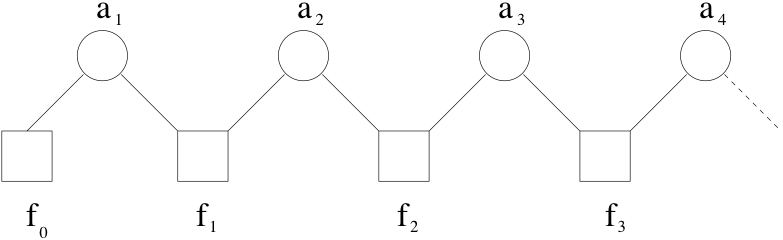
\includegraphics{images/FactorGraphExample.png}

Next, let us consider a hidden Markov model (HMM).  We can construct the 
corresponding factor graph by extending the previous example.  An HMM 
contains a Markov chain transiting from state $a_{i}$ to $a_{i+1}$. There is also an 
observation $b_{i}$ made of each state; if we are given $a_{i}$, then $b_{i}$
is conditionally independent of all other variables. We can incorporate 
this probability by using a factor:
%
\[
g_i(a_i) = Pr(b_i|a_i)
\]

The product of our factors is then
%
\begin{eqnarray*}
f_0 \left( \prod_{j=1}^{n-1} f_j(a_j,a_j+1) \right) \prod_{j=1}^n g_j(a_j)  &=& 
    Pr(a_1) \left( \prod_{j=1}^{n-1} Pr(a_{j+1}|a_j)  \right) \prod_{j=1}^n Pr(b_j|a_j)  \\
  &=& Pr(a_1,...,a_n,b_1,...,b_n)
\end{eqnarray*}

Since the $b_i$ observed, then $Pr(b_1,...,b_n)$ is a constant.  Therefore
%
\begin{eqnarray*}
Pr(a_1,...,a_n,b_1,...,b_n) & \propto & \frac{Pr(a_1,...,a_n,b_1,...,b_n)}{Pr(b_1,...,b_n)} \\
			    &=& Pr(a_1,...,a_n|b_1,...,b_n)
\end{eqnarray*}

as desired.

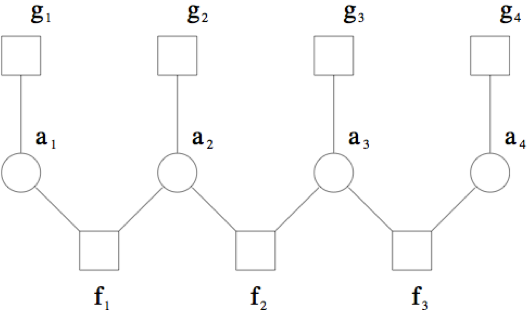
\includegraphics{images/HMMExample.png}

The resulting factor graph takes the following form illustrated in the figure above. Note 
that the variables $b_i$  need not appear explicitly in the factor graph; we have incorporated their effect in the $g_i$  factors.

Generalizing from a Markov chain to an HMM illustrates a very powerful feature of factor graphs.  Complicated mathematical models are often composed of simpler parts.  When these models are expressed as factor graphs, we can frequently reuse the simpler factor graphs to construct the more complicated ones.  This can be done simply in Dimple by using the nested graphs feature (see section~\ref{sec:nestedGraphs} on Nested Graphs).

As a final example, we will construct a factor graph for error correction (for this
 more advanced topic, we will assume the reader is familiar with LDPC codes).  Suppose
 that we receive a codeword from a 4-bit LDPC error-correcting code that has been corrupted by noise.  
The sender wishes to communicate a four-bit codeword $(a_{1},a_{2},a_{3},a_{4})$ satisfying some parity check equations, 
but the receiver only observes the corrupted values $(b_{1},b_{2},b_{3},b_{4})$. (The domain of the $b_{i}$ is determined by the 
communication channel.  For instance, if we have a discrete binary symmetric channel, then the $b_{i}$ will be bits; 
if we have a continuous additive white Gaussian noise channel and some modulation scheme, the $b_{i}$  will be real-valued.) 
Let $H$ be the parity check matrix of the LDPC code used, i.e., the codeword $(a_{1},a_{2},a_{3},a_{4})$ verifies the equation $Ha=0 \textrm{ mod } 2$.

For instance, suppose that $H$ is the following parity check matrix:
%
\[
H = \left( \begin{array}{cccc}
1 & 1 & 0 & 1 \\
1 & 1 & 1 & 0 \\
0 & 1 & 1 & 1 \end{array} \right) 
\]

Suppose that the error is independent, i.e., if we condition on $a_i$, $b_i$ is conditionally independent of the other variables.   Then, the following factor graph represents the decoding task at hand.

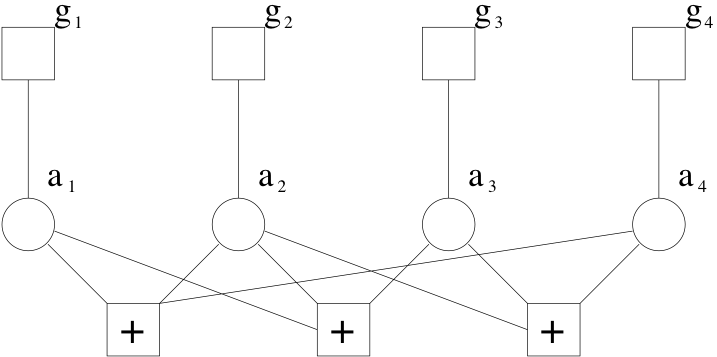
\includegraphics{images/DecoderExample.png}




The construction above applies to any linear binary ECC.  However, if every row and column of H is sparse (as would be the case with an LDPC code), then every factor is small, and every node in the factor graph will be of small degree.

Given a factor graph, the objective is often to compute the marginal distribution of the random variables $a_i$ of the graph (this also allows us to find the most likely value taken by each variable, by maximization of the marginal probability). Dimple provides an implementation of belief propagation (BP) (in its sum-product version), in order to approximately compute the marginal distribution of each random variable. 

BP is an iterative message-passing algorithm where messages pass along the edges of the factor graph.  A ``message'' can be viewed as an un-normalized probability distribution.  The algorithm comes in a number of variants depending on the message update rule and the order of the message updates.  

The sum-product form of BP generalizes a number of algorithms, including the ``forward-backward'' algorithm of HMMs, and the BCJR algorithm of coding theory. It always gives the exact answer when the underlying factor graph is a tree (if the graph contains no cycles). Although it is not an exact algorithm for general graphs, BP has been found to give excellent results for a wide variety of factor graphs, and runs particularly fast on sparse factor graphs (i.e., factor graphs of low node degree).

